\documentclass{article} % For LaTeX2e
\usepackage{nips14submit_e,times}
\usepackage{amsmath}
\usepackage{amsthm}
\usepackage{amssymb}
\usepackage{mathtools}
\usepackage{hyperref}
\usepackage{url}
\usepackage{algorithm}
\usepackage[noend]{algpseudocode}
%\documentstyle[nips14submit_09,times,art10]{article} % For LaTeX 2.09

\usepackage{bbm}
\usepackage{graphicx}
\usepackage{caption}
\usepackage{subcaption}
\usepackage{MnSymbol}

\def\eQb#1\eQe{\begin{eqnarray*}#1\end{eqnarray*}}
\def\eQnb#1\eQne{\begin{eqnarray}#1\end{eqnarray}}
\providecommand{\e}[1]{\ensuremath{\times 10^{#1}}}
\providecommand{\pb}[0]{\pagebreak}
\DeclarePairedDelimiter\ceil{\lceil}{\rceil}
\DeclarePairedDelimiter\floor{\lfloor}{\rfloor}

\newcommand{\E}{\mathrm{E}}
\newcommand{\Var}{\mathrm{Var}}
\newcommand{\Cov}{\mathrm{Cov}}
\newcommand\eqD{\stackrel{\mathclap{\normalfont\mbox{d}}}{=}}

\def\Qb#1\Qe{\begin{question}#1\end{question}}
\def\Sb#1\Se{\begin{solution}#1\end{solution}}

\newenvironment{claim}[1]{\par\noindent\underline{Claim:}\space#1}{}
\newtheoremstyle{quest}{\topsep}{\topsep}{}{}{\bfseries}{}{ }{\thmname{#1}\thmnote{ #3}.}
\theoremstyle{quest}
\newtheorem*{definition}{Definition}
\newtheorem*{theorem}{Theorem}
\newtheorem*{lemma}{Lemma}
\newtheorem*{question}{Question}
\newtheorem*{preposition}{Preposition}
\newtheorem*{exercise}{Exercise}
\newtheorem*{challengeproblem}{Challenge Problem}
\newtheorem*{solution}{Solution}
\newtheorem*{remark}{Remark}
\usepackage{verbatimbox}
\usepackage{listings}
\usepackage{mathrsfs}
\title{ProbLimI: \\
Problem Set VII}


\author{
Youngduck Choi \\
CIMS \\
New York University\\
\texttt{yc1104@nyu.edu} \\
}


% The \author macro works with any number of authors. There are two commands
% used to separate the names and addresses of multiple authors: \And and \AND.
%
% Using \And between authors leaves it to \LaTeX{} to determine where to break
% the lines. Using \AND forces a linebreak at that point. So, if \LaTeX{}
% puts 3 of 4 authors names on the first line, and the last on the second
% line, try using \AND instead of \And before the third author name.

\newcommand{\fix}{\marginpar{FIX}}
\newcommand{\new}{\marginpar{NEW}}

\nipsfinalcopy % Uncomment for camera-ready version

\begin{document}


\maketitle

\begin{abstract}
This work contains solutions to the exercises of the problem set V. The
chosen problems are 1,2, and 3.
\end{abstract}

\bigskip

\begin{question}[2]
\hfill
\begin{figure}[h!]
  \centering
    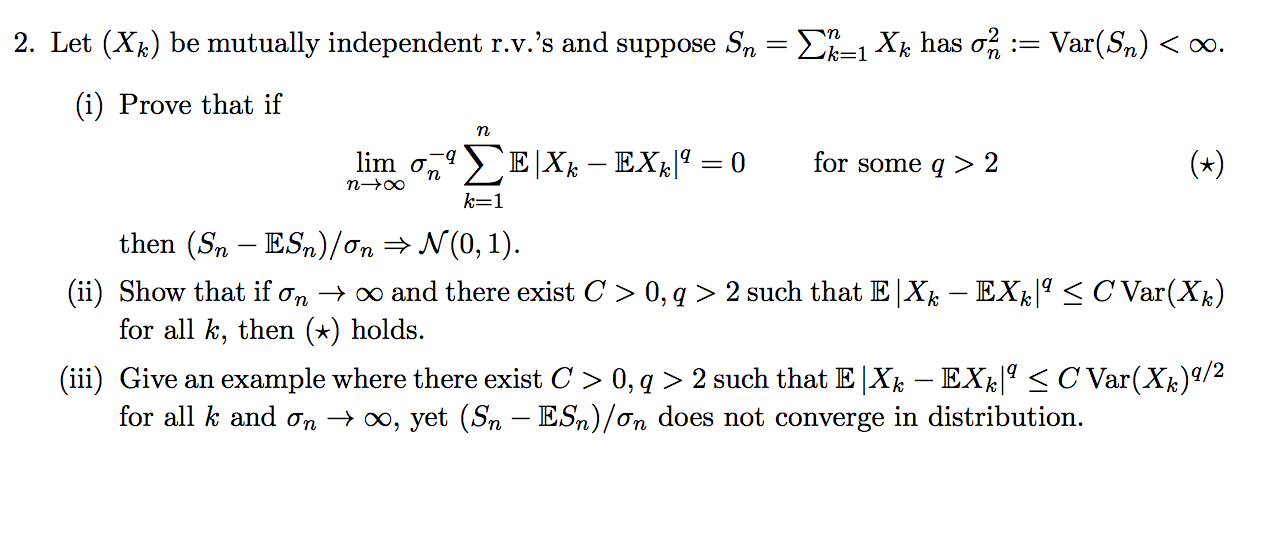
\includegraphics[width=0.7\textwidth]{prob-e7-p2.png}
\end{figure}
\end{question}
\begin{solution} \hfill \\
\textbf{(i)}
We verify the Lindenberg condition on $\{\dfrac{S_n - \mathbb{E}[S_n]}{\sigma_n}\}$.
Observe that
\eQb
\dfrac{S_n - \mathbb{E}[S_n]}{\sigma_n} = \dfrac{1}{\sigma_n} \sum_{k=1}^{n} 
X_k - \mathbb{E}[X_k] = 0 
\eQe
and 
\eQb
\mathbb{E}[\dfrac{X_k - \mathbb{E}[X_k]}{\sigma_n}] &=& 0
\eQe 
for each $n,k \in \mathbb{N}$. Furthermore,
\eQb
\sum_{n=1}^{\infty} \mathbb{E}[\dfrac{(X_k - \mathbb{E}[X_k])^2}{\sigma_n^2}] 
&=& \lim_{n \to \infty} \dfrac{1}{\sigma_n^2} \sum_{k=1}^{n} \text{Var}[X_k] = 
\lim_{n \to \infty} \dfrac{1}{\sigma_n^2} \text{Var}[S_n] = 1.
\eQe
Hence, it now suffices to show the integral condition. Fix $\epsilon > 0$. With
the given $q >2$, 
\eQb
\sum_{k=1}^{n} \mathbb{E}[\dfrac{(X_k - \mathbb{E}[X_k])^2}{\sigma_n^2} 
1_{\{|\frac{X_k - \mathbb{E}[X_k]}{\sigma_n}| > \epsilon\}}]  
&=& 
\dfrac{1}{\sigma_n^2}
\sum_{k=1}^{n} \mathbb{E}[(X_k - \mathbb{E}[X_k])^2] 
1_{\{|X_k - \mathbb{E}[X_k]| > \epsilon \sigma_n\}}] \nonumber \\
&\leq&  
\dfrac{1}{\sigma_n^2} \sum_{k=1}^{n} \mathbb{E}[(\dfrac{|X_k - \mathbb{E}[X_k]|}{
\epsilon \sigma_n})^{q-2} (X_k - \mathbb{E}[X_k])^2] 
1_{\{|X_k - \mathbb{E}[X_k]| > \epsilon \sigma_n\}}] \\
&=& 
\epsilon^{2-q} \dfrac{1}{\sigma_n^q} \sum_{k=1}^{n} \mathbb{E}[
({|X_k - \mathbb{E}[X_k]|})^{q} 
1_{\{|X_k - \mathbb{E}[X_k]| > \epsilon \sigma_n\}}] \\
&\leq& 
\epsilon^{2-q} \dfrac{1}{\sigma_n^q} \sum_{k=1}^{n} \mathbb{E}[
({|X_k - \mathbb{E}[X_k]|})^{q}]
\eQe
for any $n \in \mathbb{N}$.
Now, by the assumption, the last term goes to $0$ as $n \to \infty$. Since $\epsilon
> 0$ was arbitrary, we have shown that the desired Lindenberg condition,
Therefore, by Lindenberg CLT,
\eQb
\dfrac{S_n - \mathbb{E}[S_N]}{\sigma_n} \to_{D} N(0,1) 
\eQe
as required.  

\bigskip

\textbf{(ii)} By independence, with the given $C > 0$ and $q > 2$,
\eQb
\sigma_n^{-q} \sum_{k=1}^{n} \mathbb{E}|X_k - \mathbb{E}[X_k]|^q &\leq& 
C \sigma_n^{-q} \sum_{1}^{n} \text{Var}[X_k] = C\sigma_n^{2-q}
\eQe 
for any $n \in \mathbb{N}$. Since $2-q>0$ and $\sigma_n \to \infty$ as $n \to \infty$,
the RHS converges to $0$ as $n \to \infty$. Hence, $(*)$ holds. 

\bigskip

\textbf{(iii)} Let $\mathbb{P}(X_k = a_k) = \mathbb{P}(X_k = -a_k) = \dfrac{1}{2}$
for all $k \geq 1$, where $\{a_k\}$ are positive numbers to be chosen. We compute
\eQb
\mathbb{E}[X_k] = 0, \>\> \mathbb{E}|X_k|^q = a_k^{q}
\eQe 
so with $C=1$ and $q >2$, 
\eQb
\mathbb{E}|X_k - \mathbb{E}X_k|^q = c(\text{Var}(X_k))^{\frac{q}{2}} 
\eQe
for all $k \geq 1$. Note that, by independence,
\eQb
\sigma_n^2 = \text{Var}(S_n) = \sum_{k=1}^{n} a_k^2 \>\>\> \mathbb{E}|X_k|^3 < \infty.
\eQe
By the estimate in Durrett 3.3.8,
\eQb
\phi_{X_k}(\dfrac{t}{\sigma_n}) &=& 1 - \dfrac{a_k t^2}{2\sigma_n^2} + \Theta(\dfrac{1}
{\sigma_n^3})  
\eQe
for all $n \geq 1$, and hence
\eQb
\phi_{\sigma_n^{-1} S_n}(t) &=& \prod_{k=1}^{n} (1 - \dfrac{a_k t^2}{2\sigma_n^2} 
+ \Theta(\dfrac{1}{\sigma_n^3}) \\
&=& \exp(\sum_{k=1}^{n} \log(1 - \frac{a_k^2 t^2}{2\sigma_n^2} + \Theta(\frac{1}{
\sigma_n^3})) \\
&=& \exp(\sum_{k=1}^{n} - \frac{a_k^2 t^2}{2\sigma_n^2} + \Theta(\frac{1}{
 \sigma_n^3})) = \exp(-\dfrac{t^2}{2} + \Theta(\dfrac{n}{\sigma_n^3}))  
\eQe
for all $n$ large enough. The theta estimate comes from the fact that 
we have values less than 1 in absolute value, so we can consider a geometric
series to sum the remainder term.
Choose $\{a_n\}$ such that $\sum_{k=1}^{n} a_k^2 = \sqrt{n}$
for all $n$. Then, by the above estimate, we see that the characteristic function
diverges, so it does not converge in distribution, and we have the desired 
construction. \hfill $\qed$

\end{solution}

\newpage

\begin{question}[3]
\hfill
\begin{figure}[h!]
  \centering
    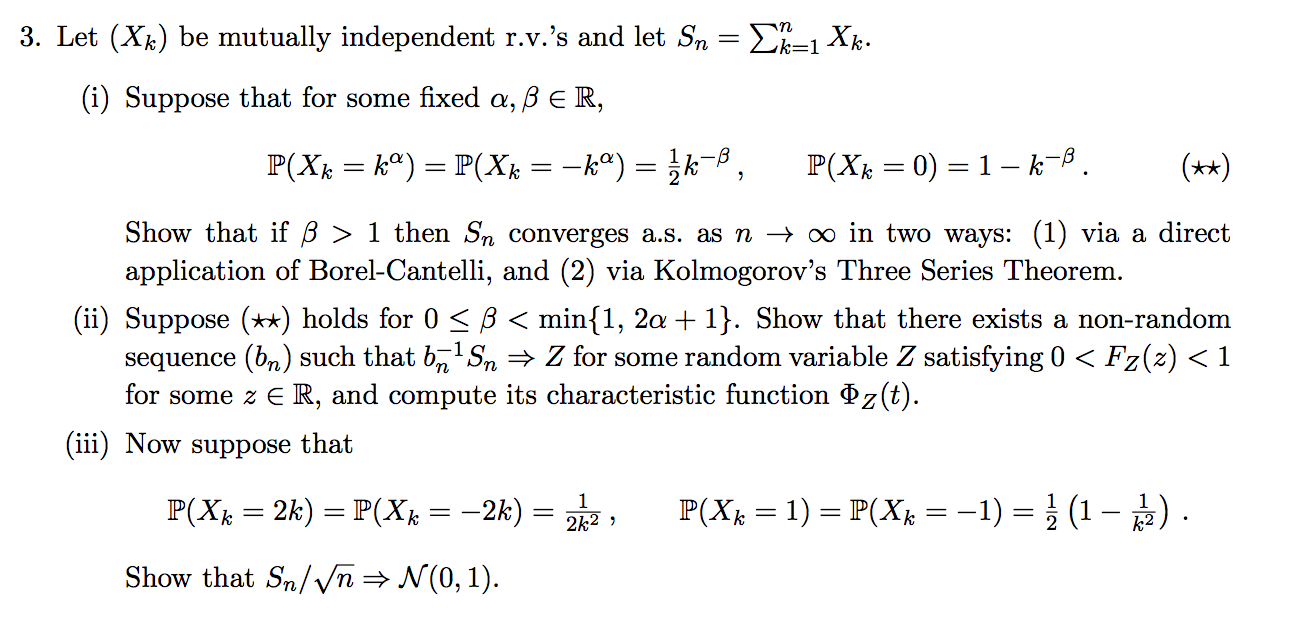
\includegraphics[width=0.7\textwidth]{prob-e7-p3.png}
\end{figure}
\end{question}
\begin{solution} \hfill \\
\textbf{(i)}
Suppose $\beta > 1$. Choose any $ 0 < C < 1$. Then,
as $|k^{\alpha}| \geq 1 > C$ for all $k \in \mathbb{N}$, 
\eQb
\sum_{k=1}^{\infty} \mathbb{P}(|X_k| \geq C) &=& \sum_{k=1}^{\infty}\mathbb{P}(
|X_k| = k^{\alpha} ) + \mathbb{P}(|X_k| = -k^{-\alpha}) 
= \sum_{k=1}^{\infty} k^{-\beta} < \infty.
\eQe 
Let $Y_k = X_k 1_{|X_k| \leq C}$ for each $k \in \mathbb{N}$. Then, as before,
\eQb
\mathbb{E}[Y_k] = 0 \>\> \text{for all} \>\> k \in \mathbb{N}
\eQe
and hence
\eQb
\sum_{k=1}^{\infty} \mathbb{E}[Y_k] < \infty.
\eQe
Similarly, 
\eQb
\text{Var}[Y_k] &=& \mathbb{E}[{Y_k}^2] - \mathbb{E}[Y_k]^2 = 0 
\eQe
for all $k \in \mathbb{N}$, so
\eQb
\sum_{k=1}^{\infty} \text{Var}[Y_k] \>\>\> \text{converges}.
\eQe
Therefore, by Kolmogorov's three series theorem, we have that $S_n$ converges a.s.

\bigskip

Choose any $0 < C < 1$. Then, 
\eQb
\mathbb{P}(|X_k| > \epsilon) = k^{-\beta} 
\eQe 
for all $k \geq 1$, and hence with $\beta > 1$,
\eQb
\sum_{k=1}^{\infty} \mathbb{P}(|X_k| > \epsilon) \>\>\> \text{is summable}.
\eQe
Hence, by BC I,
\eQb
\mathbb{P}(|X_k| \leq \epsilon \>\> \text{a.a.}) &=& 1.
\eQe
Since 
\eQb
\{ |X_k| \leq \epsilon \>\> \text{a.a.} \} \subset \{ \dfrac{S_n}{n} \>\> \text{
converges} \},
\eQe
we are done.

\bigskip

\textbf{(ii)} Suppose $0 \leq \beta < \min(1,2\alpha + 1)$. Observe that 
\eQb
\sigma_k^2 &=& \text{Var}[X_k] = \mathbb{E}[X_k^2] = k^{2\alpha-\beta} 
\eQe
for all $k \in \mathbb{N}$. Then, we have the third moment is 0 and the fourth 
moment is finite. Analogous to the solution in 2-iii, 
\eQb
\phi_{b_n^{-1} S_n}(t) &=& \exp(\sum_{k=1}^{n} \dfrac{k^{2\alpha - \beta}t^2}{
2b_n} + \Theta(\dfrac{n}{b_n^4})) 
\eQe 
Choose $\{b_n\}$ such that
\eQb
\dfrac{n}{b_n^4} \to 0 \>\>\> \sum_{k=1}^{n} k^{2\alpha - \beta} b_n^{-1} \to C
\eQe
for some $C > 0$. Then, $b_n^{-1}S_n \to_{D} N(0,C)$. So we are done.

\bigskip

\textbf{(iii)} With the exact same calculation as above, we see that 
$\phi_{\frac{S_n}{\sqrt{n}}} \to e^{-\frac{t^2}{2}}$. Therefore, we see that
it should converge to normal distribution with $0$ mean, but with variance 5.

\hfill $\qed$
 
\end{solution}

\newpage

\begin{question}[4]
\hfill
\begin{figure}[h!]
  \centering
    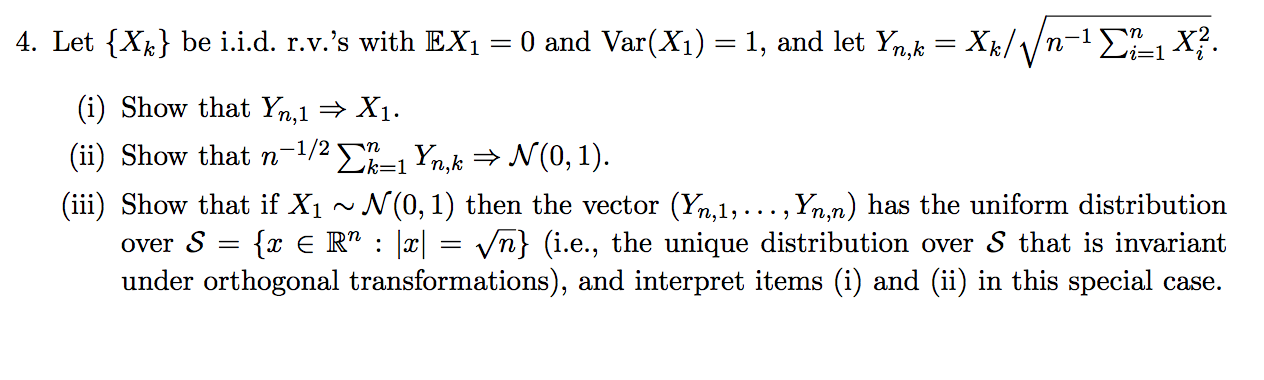
\includegraphics[width=0.7\textwidth]{prob-e7-p4.png}
\end{figure}
\end{question}
\begin{solution} \hfill \\
\textbf{(i)} By SLLN,
\eQb
\dfrac{1}{n}\sum_{i=1}^{n} X_i^{2} \to 1 \>\>\> \text{almost surely}
\>\>\> \text{and} \>\>\>
(\dfrac{1}{n}\sum_{i=1}^{n} X_i^{2})^{\frac{1}{2}} \to 1 \>\>\> \text{almost surely}
\eQe
which implies 
\eQb
Y_{n,1} = \dfrac{X_1}{(n^{-1}\sum_{i=1}^{n} X_i^2)^{\frac{1}{2}}}
 \to X_1 \>\>\> \text{almost surely}. 
\eQe
Since a.s. convergence implies convergence in distribution,
\eQb
Y_{n,1} \to_{D} X_1, 
\eQe
as required.

\bigskip

\textbf{(ii)} By CLT, 
\eQb
n^{-\frac{1}{2}}\sum_{k=1}^{n} X_k \to_{D} N(0,1).
\eQe 
Observe that
\eQb
n^{-\frac{1}{2}}\sum_{k=1}^{n} Y_{n,k} - n^{-\frac{1}{2}}\sum_{k=1}^{n} X_k 
&=& (n^{-\frac{1}{2}}) 
\sum_{k=1}^{n} X_k (\dfrac{1}{\sqrt{n^{-1}\sum_{i=1}^{n}X_i^2}} - 1) \\
&=& (\dfrac{1}{\sqrt{n^{-1}\sum_{i=1}^{n}X_i^2}} - 1)
\sum_{k=1}^{n} \dfrac{X_k}{n^{-\frac{1}{2}}} 
\eQe
for all $n \in \mathbb{N}$. By SLLN and CLT,
\eQb
(\dfrac{1}{\sqrt{n^{-1}\sum_{i=1}^{n}X_i^2}} - 1) \to_{p} 0 \>\>\> &\text{and}&
\>\>\> \sum_{k=1}^{n} \dfrac{X_k}{n^{-\frac{1}{2}}} \to_{D} N(0,1). 
\eQe
Therefore, by the result from the problem set 4 (1-iii), 
\eQb
n^{-\frac{1}{2}}\sum_{k=1}^{n} Y_{n,k} - n^{-\frac{1}{2}}\sum_{k=1}^{n} X_k \to_{D} 0. 
\eQe
Now, by the result from th problem set 4 (1-ii),
\eQb
n^{-\frac{1}{2}}\sum_{k=1}^{n} Y_{n,k} \to_{D} N(0,1) \\
\eQe
as required. \hfill $\qed$
 
\bigskip

\textbf{(iii)} Consider the distribution induced by $(X_1,...,X_n)$, which is a 
multivariate Gaussian. By symmetry of the multivariate Gaussian, we know that
the value of the distribution only depend on the distance away from the origin. Since
$(Y_{n,1},...,Y_{n,n})$ are obtained by the normalization, we see that the vector 
gives distribution that is invariant under orthogonal transformations. The measure is
unique, because we can form a product measure with a Lebesgue measure on $(0,\infty)$.
and that will give rise to Lebesgue measure on $\mathbb{R}^{n+1}$ by 
polar decomposition. Hence, for any $A \subset S^n$ measurable, $\mu(A) = m(A \times 
(0,1))$, where $\mu$ is the measure we have on $S^n$. $(i)$ is one dimensional case.
$(ii)$ is the avg value with $\sqrt{n}$
scaling of the uniform distribution, so by CLT goes to $N(0,1)$. \hfill $\qed$ 


\end{solution}
\end{document}
